\section{Results}
\label{sec:chap_slam_results}


In this section, we use the algorithm previously described~\citep{Steder2011b} to evaluate place recognition performance. We first explain how we produce the data for this evaluation and discuss about some general observations about the results for our three datasets. We then analyze the results between the unstructured and structured environments as well as between the SICK and the Velodyne acquisitions. 

\subsection{Data and General Observations}
\label{ssec:chap_slam_performance_evaluation}

In order to evaluate the place recognition performance, two elements are required. Firstly, a rule for labelling two positions of the real world as belonging---or not---to the same place, and secondly, the algorithm prediction for two input scans. In the following subsection, we first discuss these two elements and present the resulting data. Afterwards, we explain some observations about that data.


\subsubsection{Real-World Places}
As seen in previous work on topological mapping~\citep{Valgren2008, Brunskill2007} the notion of a place is ill-defined. A simple rule can be established, however: the closer two points of the space are to each other, the more likely they are to be considered in the same place. Therefore, we use the real world physical distance between two acquisitions ($d$) as an indicator of the likelihood that they represent the same place. We will now discuss the method used to determine the distance between scans. 

We first use the robot wheel odometry as a rough approximation of the relative pose between two consecutive scans. In order to reduce the pose estimation error, we then use the \gls*{icp} algorithm to align their respective point clouds and adjust the odometry accordingly. These steps are performed sequentially for all scans of the first loop. This process cannot be repeated independently for the second loop, because the drift accumulation would differ from loop to loop. The result would be that the calculated physical distance between a point in the first loop and its (true) corresponding point in the second loop might be significantly erroneous. To address this problem, the \gls*{icp} odometry adjustment of the second loop is performed relative to the first loop, thus ensuring that this difference in drift do not happen. To do this, we first align the first scan of the second loop relative to the first scan of the first loop using \gls*{icp}. Thereafter, each scan of the second loop is adjusted with respect to the scan of the first loop, that theoretically is being the closest, considering the last corrected pose and the movement of the robot. Figure~\ref{fig:chap_slam_results_paths} illustrates the resulting pair of paths for each of our three datasets. Note that this is a \gls*{2d} representation for which the vertical component is ignored. This figure shows the absence of discrepancy between the two loops of each dataset.

With the corrected odometry, it is possible to easily obtain the distance between two scans. To do this, one can simply calculate the norm of the difference in position between the two scans. On the other hand, it is important to remember that there is an accumulation of drift in the computed odometry, making the final loop slightly deformed (visible in Figure~\ref{fig:chap_slam_results_paths} \protect\subref{fig:forest_paths} \protect\subref{fig:velodyne_paths}). This results in a significant error on the estimated distance between two scans ($scan_i$ and $scan_j$, where $i<j$) that are separated by several acquisitions; for instance, between the first scan and the last scan. To address this problem we consider a new path going from $scan_j$ to $scan_i$, in addition to the previously computed path going directly from $scan_i$ to $scan_j$. This new path must pass through the loop closure portion (i.e. the link between the last scan and the first scan). Again, we used \gls*{icp} to calculate this portion of the path. Finally, the path for which the scans are closest in terms of acquisition numbers, from $scan_i$ to $scan_j$ or from $scan_j$ to $scan_i$, is used for the final calculation of the distance.

Note that all alignment is visually inspected to ensure that \gls*{icp} had indeed converged to a valid solution. When this is not the case, the odometry provided by the robot is manually adjusted to enable this convergence. The second row of Figure~\ref{fig:chap_slam_results} contains the resulting distance matrices for all pairs of scans of each of our three datasets. Note that since a distance function is by definition symmetrical, the distance matrices are symmetric by definition. The values on the main diagonal represent the distance between a scan and itself and are therefore null. A secondary diagonal of low values is produced by the small distances between the scans ($d$) of the first and the second loop. Finally, because we tried to stop the loop acquisitions approximately at the starting point, we observe small values at those junction points (at the bottom left corner of the distance matrix for instance).

\begin{figure}
    \centering
    \subfloat[]{\label{fig:building_paths}}{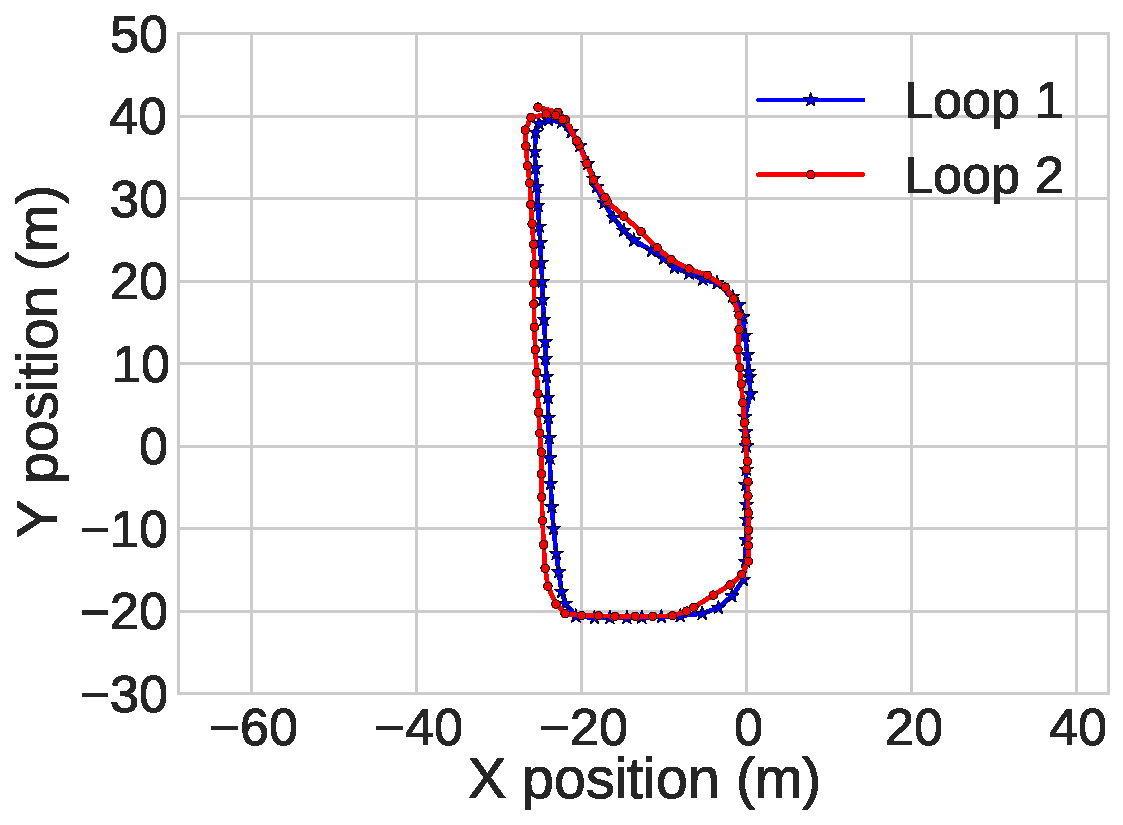
\includegraphics[width=0.45\linewidth]{img/chap_slam/building_paths.pdf}}
    \subfloat[]{\label{fig:forest_paths}}{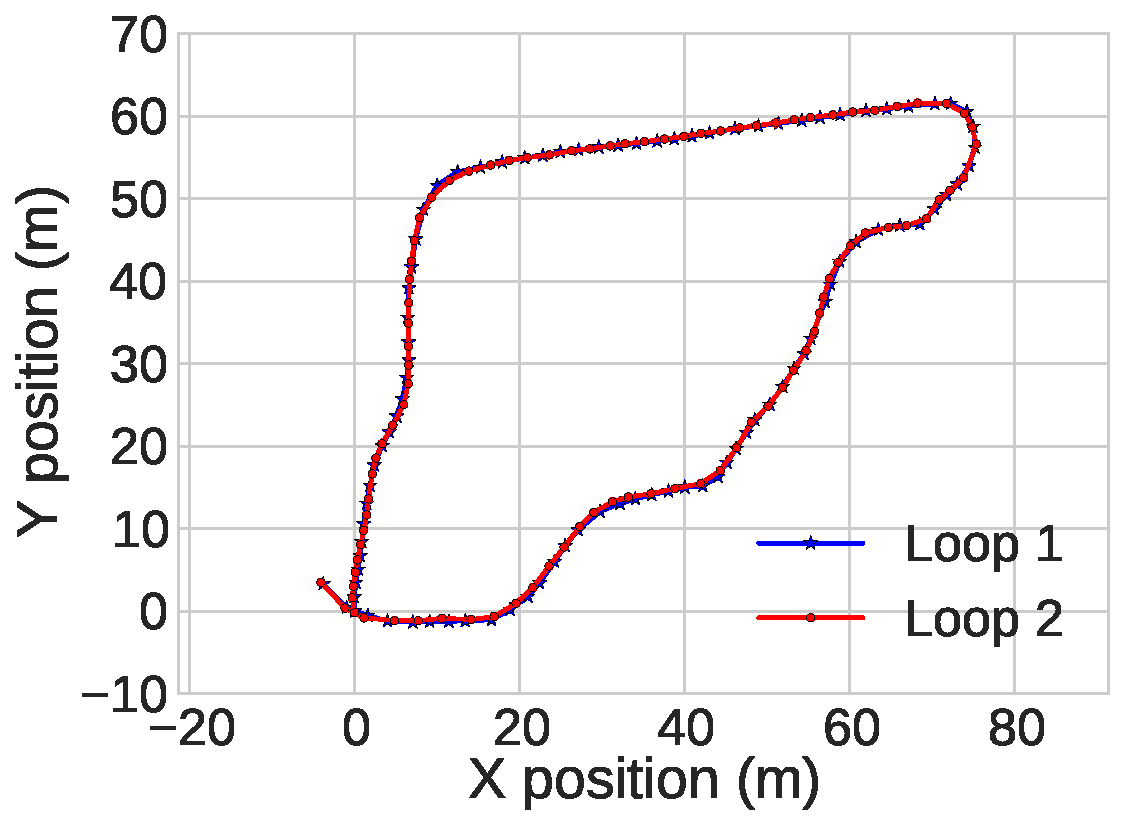
\includegraphics[width=0.45\linewidth]{img/chap_slam/forest_paths.pdf}}
    \subfloat[]{\label{fig:velodyne_paths}}{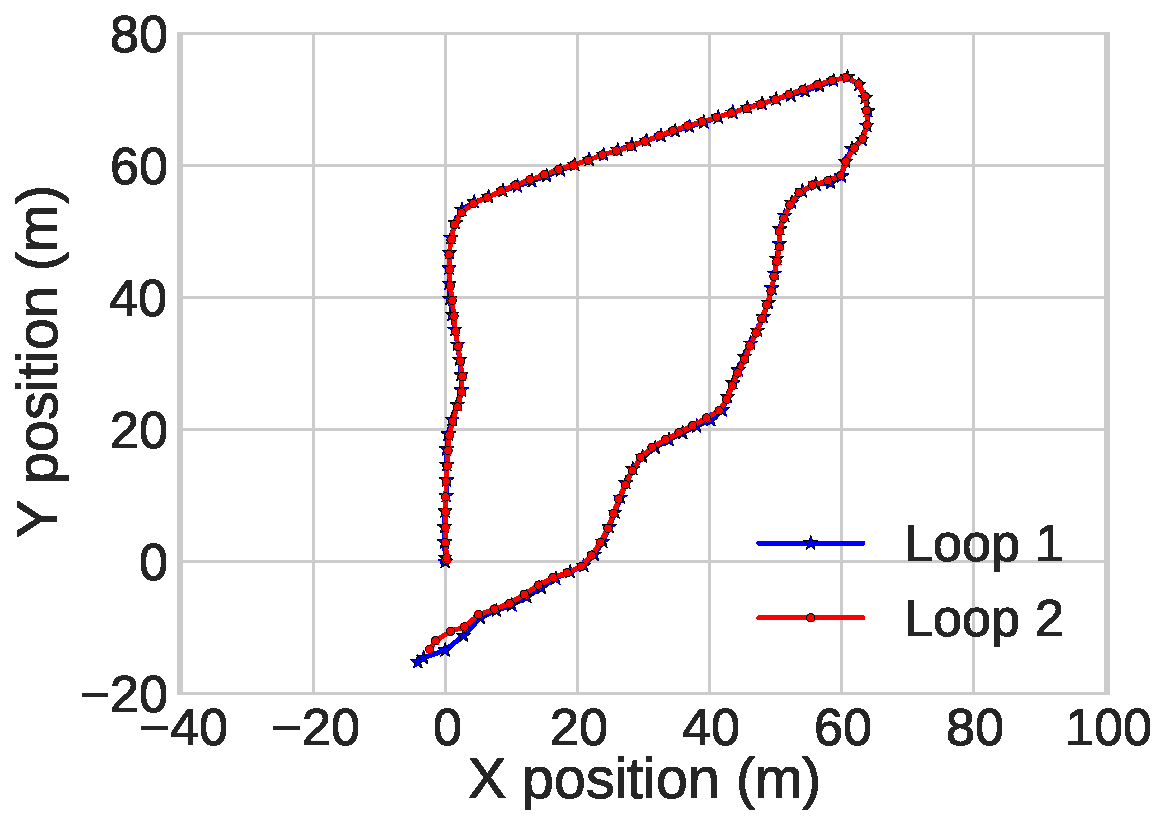
\includegraphics[width=0.45\linewidth]{img/chap_slam/velodyne_paths.pdf}}
    \caption[Path adjusted using \gls*{icp} for our three datasets.]{The path resulting from the odometry adjusted with \gls*{icp} for the two loops of each of our three datasets. \protect\subref{fig:building_paths} shows the path for the \texttt{Structured-SICK} dataset, \protect\subref{fig:forest_paths} shows the path for the \texttt{Unstructured-SICK} dataset and \protect\subref{fig:velodyne_paths} shows the path for the \texttt{Unstructured-Velodyne} dataset. Note that each marker represents the location of an acquisition.}
    \label{fig:chap_slam_results_paths}
\end{figure}


\subsubsection{Algorithm Prediction}
For our experiments, we use a \textit{C++} implementation of the place recognition algorithm developed by~\citet{Steder2011b}, who gratefully provides us with the source code. The software produce a score between 0~and~1 for each pair of scans in the database. As explained in Section~\ref{sec:chap_slam_algo}, this score reflects the system belief that two scans represent the same place. More precisely, when the score is zero, the algorithm believes there is no chance that the scans originate from the same place, and when the score is one, the algorithm is certain that they do not originate from the same place.

The second row of Figure~\ref{fig:chap_slam_results} represents the scores matrices for our three datasets. Note that the main diagonal of these matrices are the scores of a scan compared to itself, which always results in a value of~1. It is possible to observe a slight asymmetry in the matrices caused by the non-symmetric function used for calculating scores. Note that, for our results analysis, we only consider the values from the area below the main diagonal.


\subsubsection{General Observations}
\label{ssec:chap_slam_results_evaluation}

Considering the two previous subsections, we should expect to see a high score for a pair of scans close to each other and a low score for a pair of distant ones. This relationship can actually be observed by the similarity of diagonal patterns between the distances matrices and the scores matrices (first and second rows of Figure~\ref{fig:chap_slam_results}). The third row of Figure~\ref{fig:chap_slam_results} illustrates this relation with a scatter plot, where each pair of scans is represented by a single data point relating the physical distance between the scans ($d$) and the score produced by the place recognition algorithm. The set of data points seems to follow a function of the form $f(x) = 1 / x$, which also confirms our intuition.

While it is interesting to observe the complete continuous relationship between these values, practical uses of place recognition generally require a binary labelling of each pair of scans (either originating from the same place or not). To determine the ground truth labels (real-world places), a threshold $T_{distance}$ is defined on the distance between the scans ($d$). All pairs of scans closer than $T_{distance}$ is considered as being in the same place. Similarly for the algorithm predictions, a threshold $T_{score}$ is used in conjunction with output score. All pair of scans obtaining a score higher than this threshold $T_{score}$ is labelled as a match (i.e. the scans originate from the same place). Table~\ref{tab:chap_slam_results_labeling} summarizes how these two thresholds are used to label data and analyze results. Note that $T_{distance}$, as opposed to $T_{score}$, $T_{distance}$ is not a parameter of the place recognition system, but rather a tool for quantifying results. 

\begin{table}
    \centering
    \begin{tabular}{@{}l|ll@{}}
        \toprule
                                  & $\mathbf{d < T_{distance}}$ & $\mathbf{d >= T_{distance}}$ \\
        \hline
        $\mathbf{s > T_{score}}$  & True Positive (TP)          & False Positive (FP) \\
        $\mathbf{s <= T_{score}}$ & False Negative (FN)         & True Negative (TN) \\
        \bottomrule
    \end{tabular}
    \caption[Summary of scans pairs labelling for results analysis.]{A summary of scans pairs labelling for results analysis. $d$ represents the distance between the two scans and $s$ represents the place recognition algorithm output score. $T_{distance}$ and $T_{score}$ represent the distance threshold and the score threshold, respectively.}
    \label{tab:chap_slam_results_labeling}
\end{table}

The value of $T_{distance}$ to consider during the evaluation of results depends on different factors, such as the environment in which the place recognition algorithm is used. For instance, one might consider that for indoor environments, places are generally very close from each other (e.g. closer than \SI{4}{\meter}). In our context of open outdoor environments, we consider that the value of $T_{distance}$ is mainly limited by the maximum measurement range of the sensor (i.e. approximately \SI{50}{\meter}), because over two times this measurement range, there is no possible overlap between the scans. Choosing a higher value for $T_{distance}$ implies that the robot can be further away from the previously visited place and should still be able to recognize it. Consequently, maintaining relatively high scores even for higher $T_{distance}$ values is often preferable, because it allows greater flexibility during the robot navigation. The fourth row of Figure~\ref{fig:chap_slam_results} shows how the recall decreases as $T_{distance}$ increases, which can be explained by the reduction of overlap between scans, making the place recognition task more difficult.

As indicated in the introduction of this chapter (Section~\ref{sec:chap_slam_intro}), \gls*{slam} algorithms often use place recognition to detect loop closures. When the robot detects that it is in a place visited before, it can connect (or merge) these concordant regions and adjust the map accordingly. If two scans are falsely identified as coming from the same place (i.e. a false positive), the \gls*{slam} algorithm will distort the map while trying to connect them. In contrast, if a place is not recognized (i.e. false negative), the algorithm simply does not benefit from this cue to adjust the map, without further adverse results. Therefore, false positives are significantly more harmful than false negatives (sometimes catastrophic to the point of rendering the map useless) and must be avoided. 

A solution to avoid \gls*{fp} is to rely on high-confidence matches (i.e. by choosing a score threshold that is high enough). In our experiment, the minimum values for this threshold are depicted by the line in the graphs of the third row of Figure~\ref{fig:chap_slam_results}. In other words, if $T_{score}$ is above that line for the considered value of $T_{distance}$, this will result in no \gls*{fp}. Moreover, the closer the value is from that line, the better the recall will be. In our case, the recall represents the fraction of real-world places that are correctly identified by the algorithm (i.e. $TP/(TP+FN)$). The recall is presented as function of $T_{distance}$ for different score thresholds in the fourth row of Figure~\ref{fig:chap_slam_results}. One can see that, as we pick a lower threshold value $T_{score}$, the recall rate increase, as we become more permissive for our matches. 

\begin{figure}
    \centering
    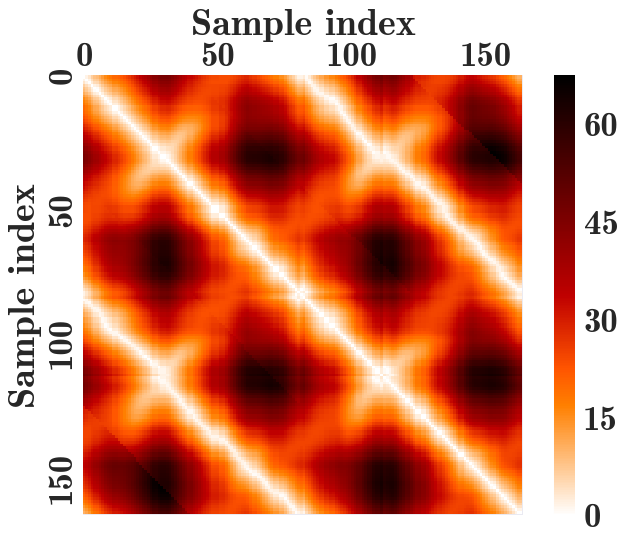
\includegraphics[width=0.32\linewidth]{img/chap_slam/building_distances_matrix.png}
    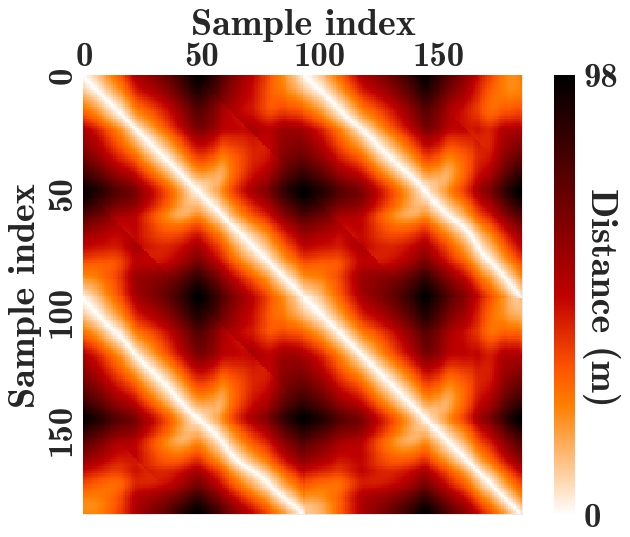
\includegraphics[width=0.32\linewidth]{img/chap_slam/forest_distances_matrix.png}
    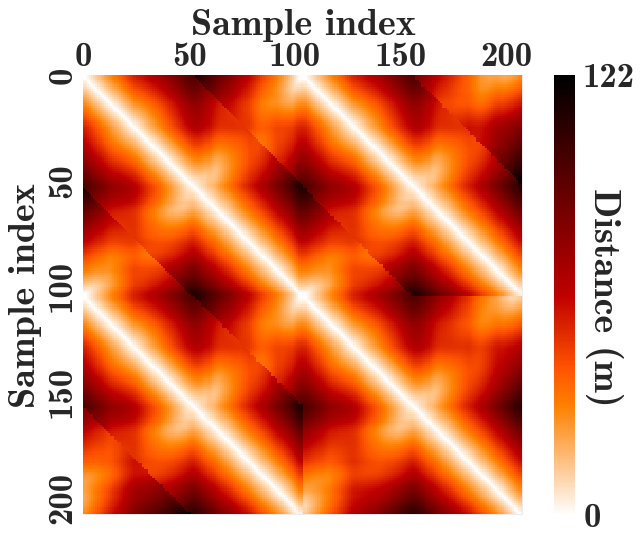
\includegraphics[width=0.32\linewidth]{img/chap_slam/velodyne_distances_matrix.png} \\

    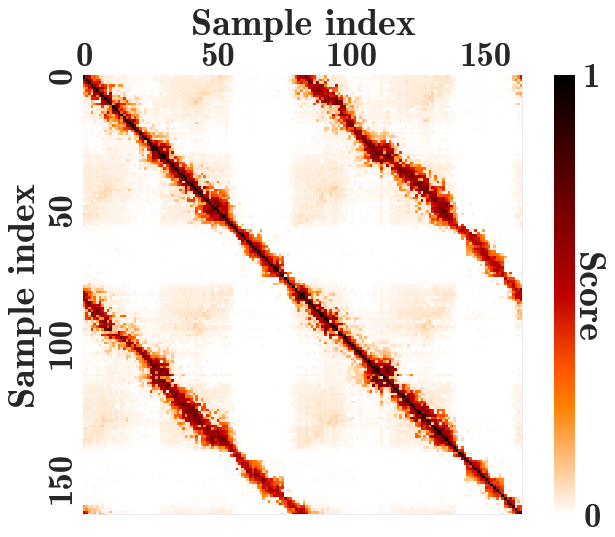
\includegraphics[width=0.32\linewidth]{img/chap_slam/building_scores_matrix.png}
    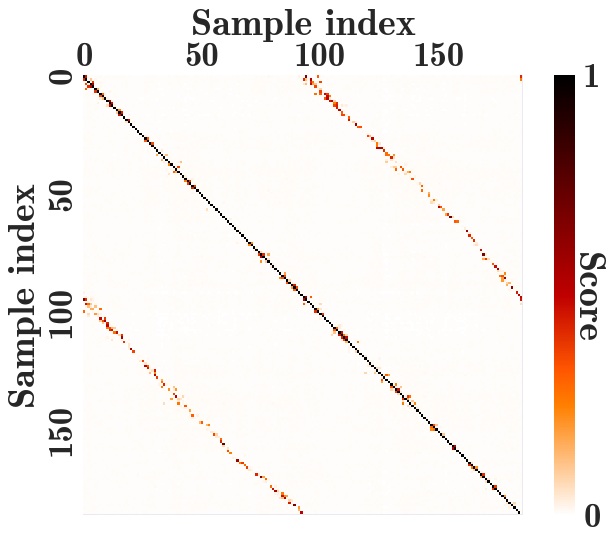
\includegraphics[width=0.32\linewidth]{img/chap_slam/forest_scores_matrix.png}
    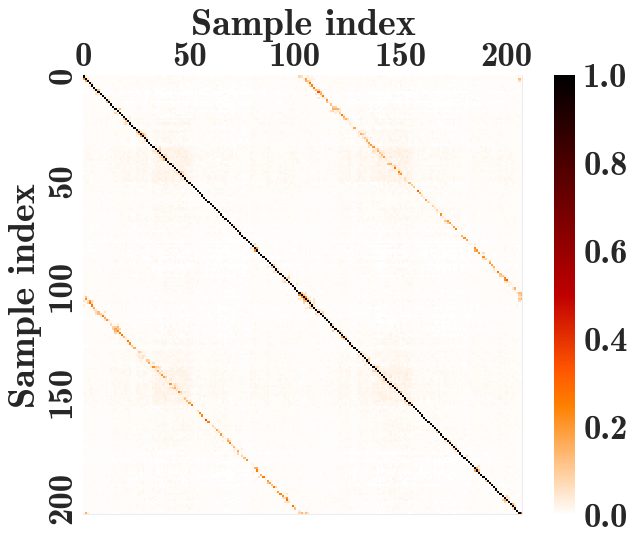
\includegraphics[width=0.32\linewidth]{img/chap_slam/velodyne_scores_matrix.png} \\

    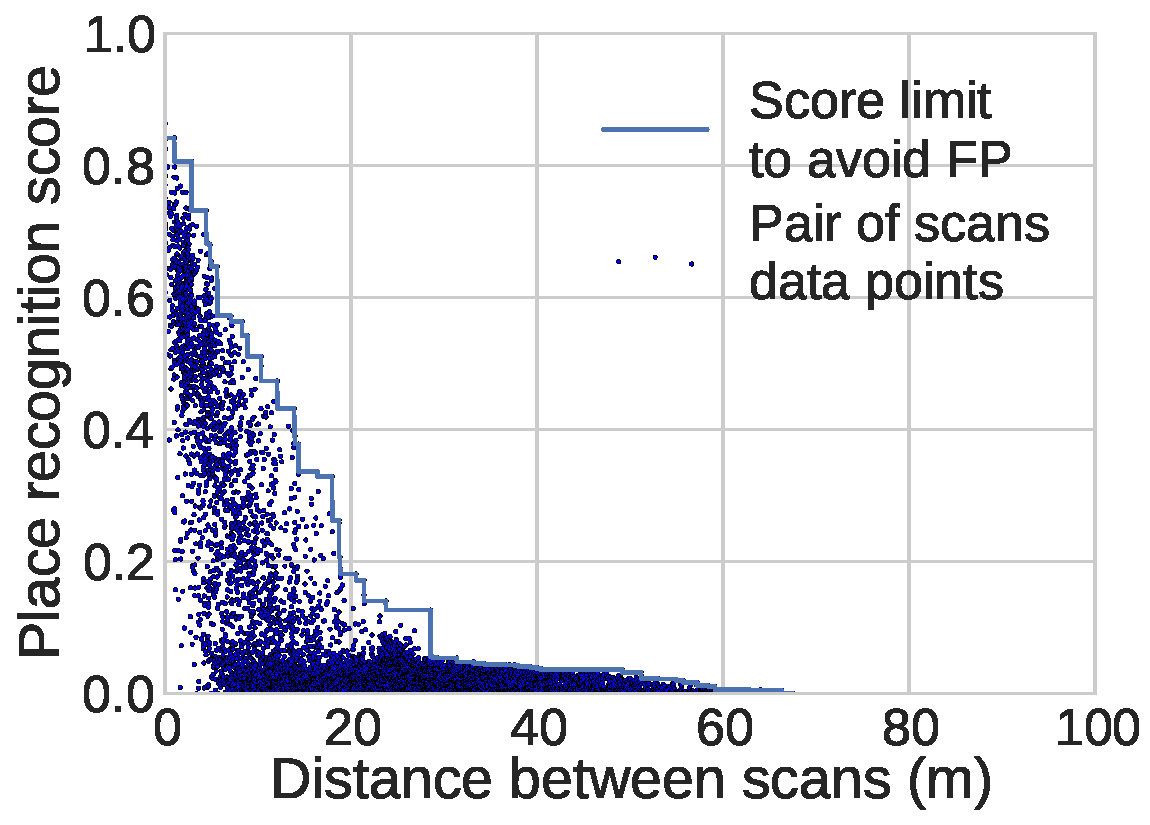
\includegraphics[width=0.32\linewidth]{img/chap_slam/building_distances_scores.pdf}
    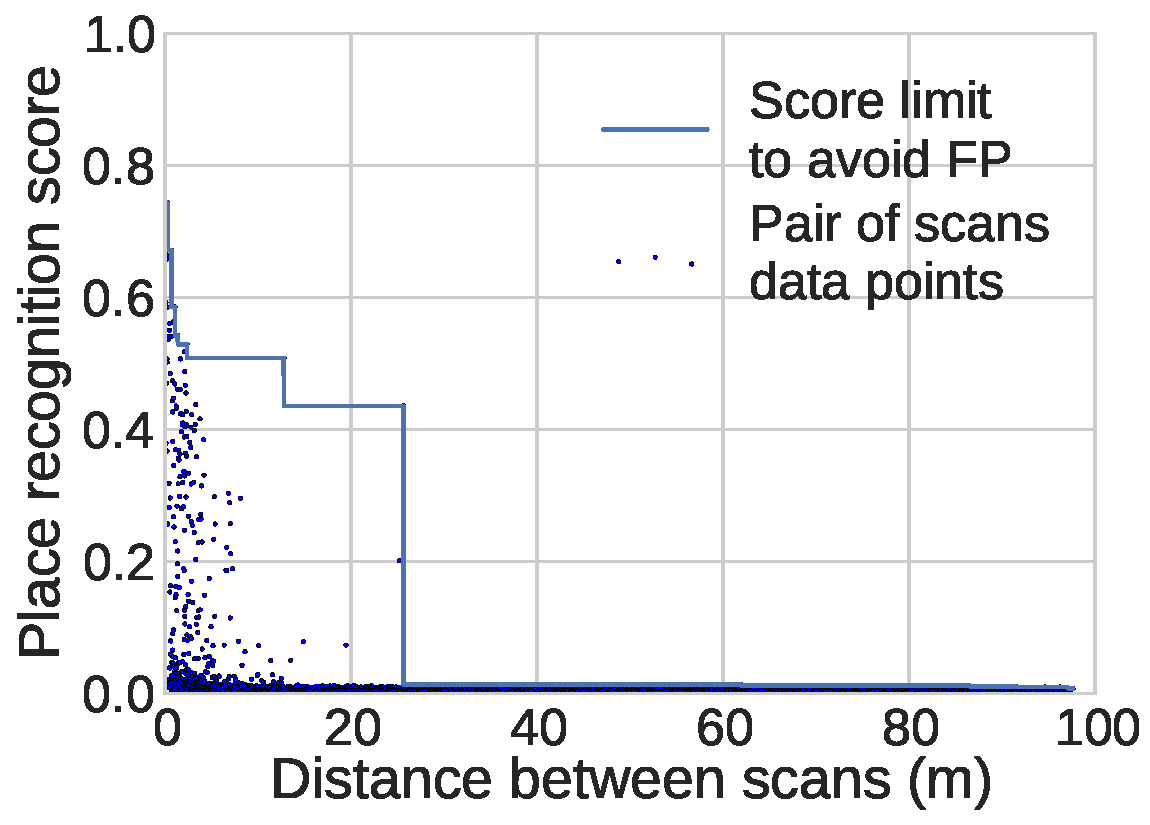
\includegraphics[width=0.32\linewidth]{img/chap_slam/forest_distances_scores.pdf}
    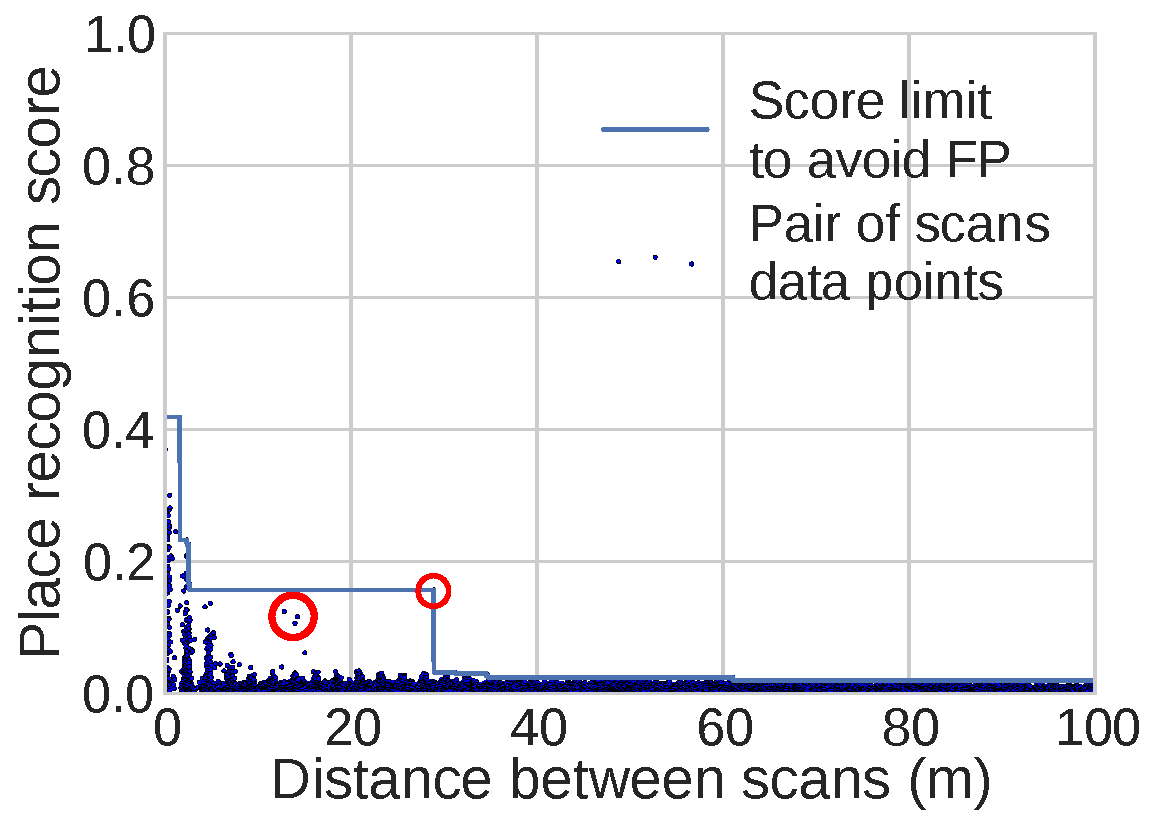
\includegraphics[width=0.32\linewidth]{img/chap_slam/velodyne_distances_scores.pdf} \\

    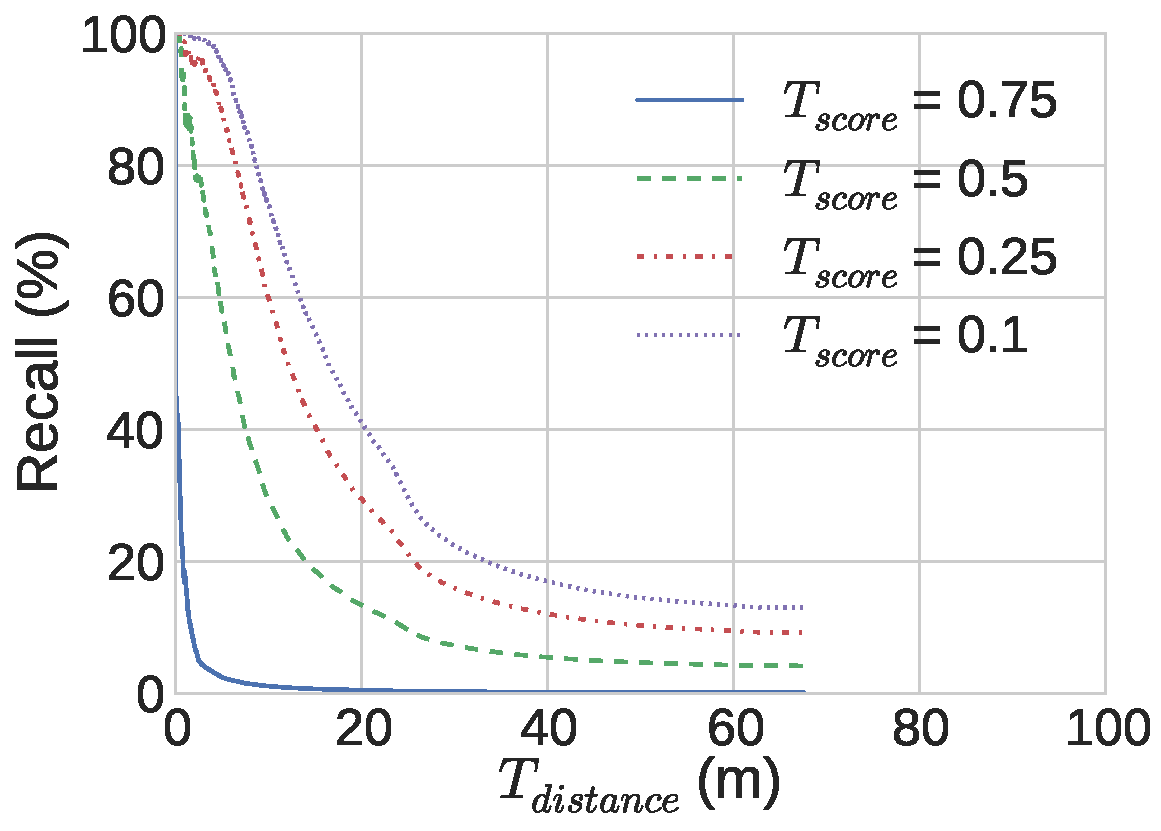
\includegraphics[width=0.32\linewidth]{img/chap_slam/building_recall.pdf}
    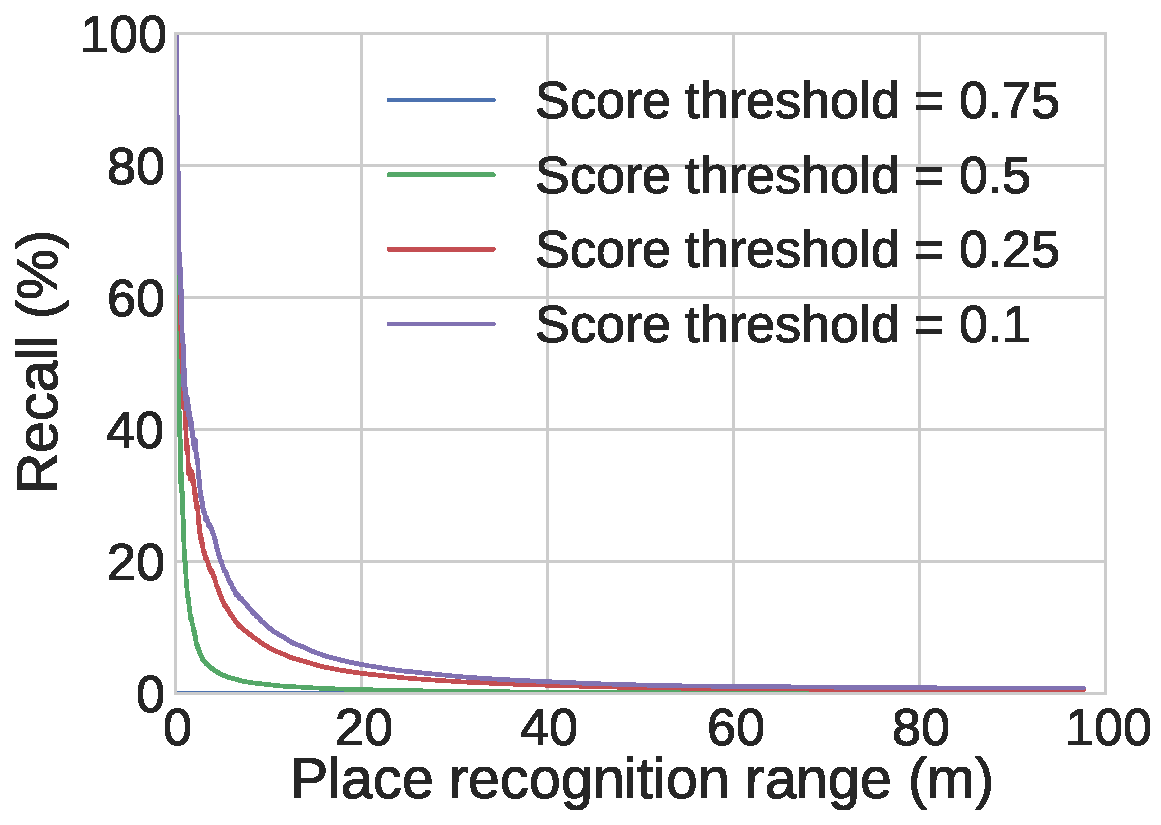
\includegraphics[width=0.32\linewidth]{img/chap_slam/forest_recall.pdf}
    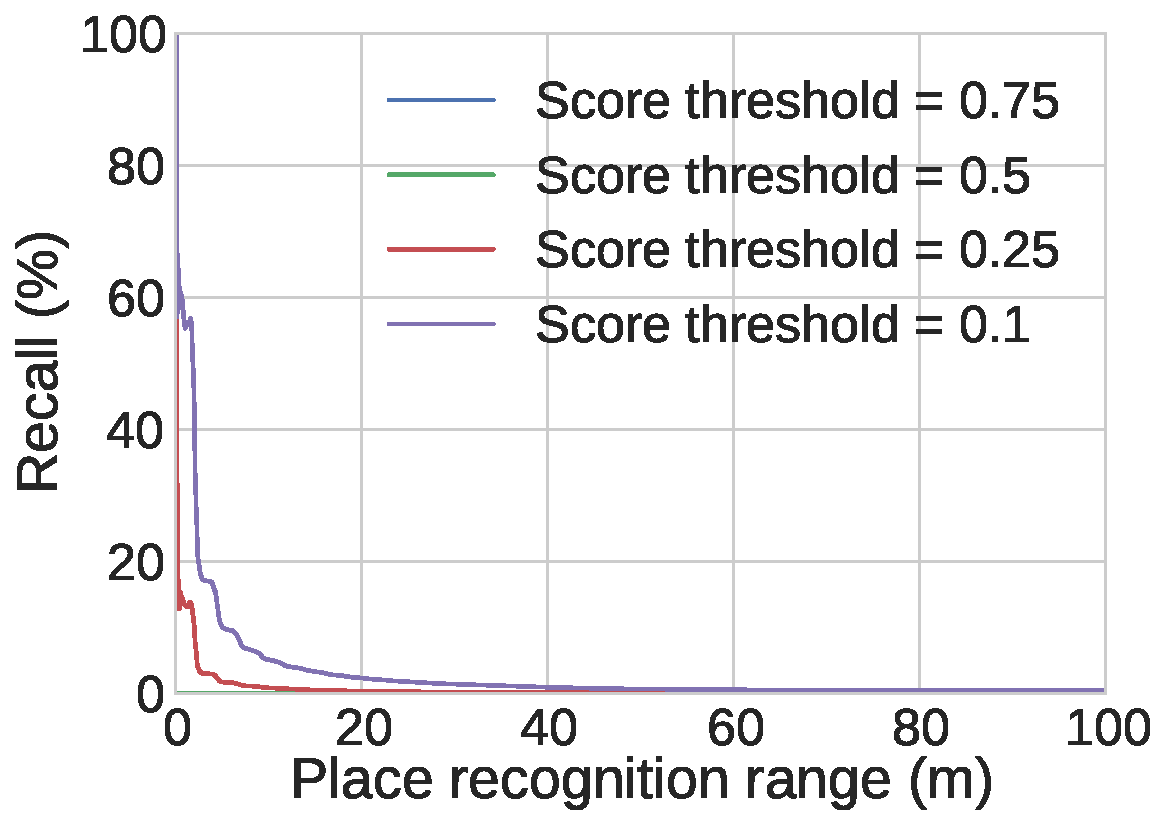
\includegraphics[width=0.32\linewidth]{img/chap_slam/velodyne_recall.pdf}

    \caption[Place recognition results overview for our three datasets.]{Place recognition results overview for our three datasets. \textbf{First column:} The \texttt{Structured-SICK} dataset. \textbf{Second column:} The \texttt{Unstructured-SICK} dataset. \textbf{Third column:} The \texttt{Unstructured-Velodyne} dataset. \textbf{First and second rows:} The matrices of distances and scores, respectively. The axes show the ordered sample indices for both loops sequentially. Consequently, all pairs of scans are represented by a position in the matrices and the colour represent the distance between the scans of a pair (first row) and the place recognition algorithm output score (second row). \textbf{Third row:} The association between the distance separating the scans and the score obtained for all scans pairs, as well as the score limit to avoid any \gls*{fp} as function of the distance between the scans. Outliers are circled in red. \textbf{Fourth row:} The recall rate as function of the maximum distance (\SI{}{\meter}) between scans to be considered as originating from the same place ($T_{distance}$).} 
    \label{fig:chap_slam_results}
\end{figure}

\subsection{Comparative Analysis}
\label{ssec:chap_slam_comparative_analysis}

In the previous subsection, we explained how we produce the results and we discussed some observations for our datasets from a general perspective. We now focus on the main interest of this document, and analyze how the algorithm behaves in the unstructured environment compared to the structured environment. We also conduct this comparative analysis between two \gls*{lidar}s, the SICK LMS151 and the Velodyne HDL-32E. For these comparisons, we consider how the score changes as function of $d$ and look for outliers. Finally, even if the current experimental configuration does not allow to determine the exact source of the differences in results, we suggest some possible causes.


\subsubsection{Structured and Unstructured Environments}
\label{ssec:chap_slam_struct_vs_forest}

%\todo{Basically, rework this paragraph... Phil doesn't think the argument is good, doesn't agree with 1/x and outliers that support the idea (I still think it is ok)}\\
For this comparison, we expect the performance of the algorithm to be worse for unstructured environments than for structured environments. Indeed, we think that the uneven ground, the significant occlusions and the presence of many small structures (e.g. branches, leaves) in unstructured environments are harmful to the \gls*{lidar}-based place recognition task. In order to evaluate this hypothesis, we look at the score as function of $d$ (third row of~\ref{fig:chap_slam_results}). As noticed previously, the distribution of points seems to represent a function of the form $f(x) = 1 / x$. In the case of the structured environment, no point appears to significantly challenge this distribution, but for the unstructured environment, there seems to be outliers (circled in red) when the value of $d$ is around \SI{13}{\meter} and \SI{25}{\meter}. To avoid getting \gls*{fp} caused by these outliers, the score threshold must be set higher, therefore reducing the recall (see Figure~\ref{fig:chap_slam_results} row four).

Another element to suggest that the performance is better in the structured environment is the value of $d$ for which the score stop decreasing significantly as the value of $d$ increase (i.e. where the distribution becomes almost horizontal). It can be observed in the third row of Figure~\ref{fig:chap_slam_results} that this happens for $d$ of approximately \SI{30}{\meter} in the structured environment and approximately \SI{15}{\meter} in the unstructured environment. For $d$ above these values, all data points are spread almost evenly under a horizontal line (i.e. score value). It is therefore impossible to discriminate pair of scans that originate from the same place from those that do not originate from the same place based on the algorithm output score. In other words, the algorithm is able to correctly identify places in a larger radius for the structured environment than in the unstructured environment.


We will now propose a few possible causes as to why the results are better in the structured environment than in the unstructured environment. As indicated in Section~\ref{sec:chap_slam_data_acquisition}, the average acquisition range is smaller for the unstructured datasets. Therefore, because of parallax, a given movement of the robot will have a greater influence on the scan content in this dataset. In addition, the unstructured environment contains many objects distributed throughout the reachable space by the \gls*{lidar}, which in conjunction with the parallax, creates many different occlusion patterns. In other words, the objects or parts of objects captured by the \gls*{lidar} greatly change as we move the robot. Another element to consider is the types of object that are present in the various environments. For instance, the objects present in the structured environment, such as buildings, are potentially better represented by the NARF features. Indeed NARF features were tested on man-made objects~\cite{Steder2011a} and in structured environments~\cite{Steder2010, Steder2011b}. Finally, because of the structured environment ground is almost entirely flat, the alignment between two scans is summed almost entirely to a translation along the XY plane and rotation about the Z axis. The additional degrees of freedom (i.e. translation along the Z axis and rotations about X and Y axis) caused by the uneven ground in the unstructured environment are likely to make the scans alignment process of the place recognition algorithm more challenging. 


\subsubsection{SICK and Velodyne \gls*{lidar}s}
\label{ssec:chap_slam_sick_vs_velodyne}

In this section, we are interested in comparing the SICK and the Velodyne performance for place recognition, as it might help understand how important the choice of the sensor is for this particular task. In our case, we expected the SICK mounted on the \gls*{ptu} to have better results for place recognition, as it retrieves more information about the scene than the Velodyne. As a reminder, Section~\ref{sec:chap_slam_data_acquisition} and more precisely in Table~\ref{tab:slam_sensor_resolution}, provide details about these sensors and the acquired data. One can notice that, although the Velodyne has a better horizontal resolution than the SICK, it has a smaller vertical resolution and \gls*{fov}, as well as a smaller total point counts (refer to Table~\ref{tab:slam_sensor_resolution}). 

Our first interesting observation, in the third row of Figure~\ref{fig:chap_slam_results}, is that all the scores obtained with the Velodyne are below $0.5$. This means that the algorithm has very low confidence that any pair of scans originate from the same place, even when those scans are very close physically from each other. In comparison, the data obtained with SICK produce scores above 0.7 for scans that are really close. Consequently, data points are concentrated in the lower part of the graph and the place recognition’s results will be more sensitive to the choice of score threshold. We can also confirm these observations with the graphics of the fourth row of Figure~\ref{fig:chap_slam_results}. There, one can see that for all of the Velodyne data, the recall is 0 when the score threshold is set to $0.75$ or $0.5$. There is also a greater gap between the two other curves (i.e for score thresholds of $0.25$ and $0.1$) over the corresponding curves for SICK.

On the other hand, there seems to be no major differences between those distributions regarding the value of $d$ for which the score stop decreasing significantly (around \SIrange{10}{15}{\meter}). One could argue that this maximum range is simply due to the closeness of the environment. In addition, it does not seem to be any significant difference in the amount or distribution of outliers, which is important to avoid \gls*{fp}.

It can be concluded that there is indeed a difference between the results obtained for these two sensors. However, this difference may be insufficient to counteract other practical factors. For instance, one could choose to use the Velodyne for its higher data throughput, despite its slightly worse performance, and thus avoid having to immobilize the robot for each acquisition.

\FloatBarrier
